\documentclass[12pt]{article}
\usepackage{circuitikz}
\usepackage{pgfplots}
\usepackage{amsmath}

\begin{document}

\section*{Analyse du Circuit RC}

\subsection*{Schéma}
\begin{center}
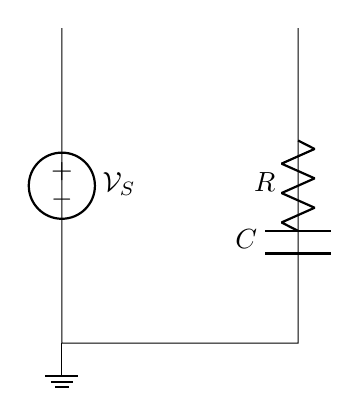
\begin{tikzpicture}[american]
\draw (0,0) node[ground]{} -- ++(0,4) to[V, l=$\mathcal{V}_S$] (0,0)
-- ++(3,0) to[R, l=$R$] (3,4) -- ++(0,-4) to[C, l=$C$] cycle;
\end{tikzpicture}
\end{center}

\subsection*{Courbe de Tension}
\begin{center}
\begin{tikzpicture}
\begin{axis}[
    xlabel={Temps (s)},
    ylabel={Tension (V)},
    xmin=0, xmax=0.01,
    ymin=0, ymax=10,
    samples=200
]
\pgfmathsetmacro{\RC}{0.005}
\addplot[blue] {10*(1-exp(-x/\RC))};
\end{axis}
\end{tikzpicture}
\end{center}

\subsection*{Équation}
\[
V_C(t) = \mathcal{V}_S \left(1 - e^{-\frac{t}{RC}}\right)
\]

\end{document}